\begin{frame}% frame 00
    \frametitle{Classic epidemic models}
    \begin{textblock*}{50mm}(5mm, 10mm)
        Consider the deterministic SI model:
        \begin{align*}
        \frac{dS}{dt} &= -\frac{\beta}{N} S I + (b +\gamma) I
        \\
        \frac{dI}{dt} &= \frac{\beta}{N} S I - (b +\gamma) I
        \\
        N &= S(t)+ I(t)
        \end{align*}
        Where $N$ is constant and  $S(t) = N - I(t)$.
    \end{textblock*}
    \only<2->{
        \begin{textblock*}{50 mm}(60mm, 10mm)
            \begin{empheq}[box=\shadowbox]{align*}
            \mathcal{R}_0 &= 
            \frac{\beta}{b + \gamma}
            \\
            \mathcal{R}_0 & \leq 1
            \\
            & \Rightarrow
            \lim_{t \to \infty} (S(t),N(t)) = (N, 0)
            \\
            \mathcal{R}_0 & > 1
            \\
            & \Rightarrow
            \lim_{t \to \infty} (S(t),N(t)) = (S^*, I^*)
            \end{empheq}
        \end{textblock*}
    }
    \only<3->{
        \begin{textblock*}{50mm}(10mm, 55mm)
            \textbf{Kermack-McKendrick Model}
            \begin{align*}
            \frac{dS}{dt} &= 
                -\beta S I 
            \\
            \frac{dI}{dt} &= \beta S I  
            \\
            \frac{dR}{dt} &= \gamma I
            N &= S(t)+ I(t) + R(t)
            \end{align*}
            Where $N$ is constan.
        \end{textblock*}
        \begin{textblock*}{60mm}(60mm, 50mm)
            \begin{empheq}[box=\shadowbox]{align*}
            \mathcal{R}_0 &= 
            \frac{\beta}{\gamma}
            \\
            \mathcal{R}_0 & \leq 1
            \\
            & \Rightarrow
            \lim_{t \to \infty} (S(t), I(t), R(t)) = (N, 0, 0)
            \\
            \mathcal{R}_0 & > 1
            \\
            & \Rightarrow
            \lim_{t \to \infty} (S(t),N(t)) = (S^*, I^*, R^*)
            \end{empheq}
        \end{textblock*}
    }
\end{frame}

\begin{frame}{}
    \begin{center}
        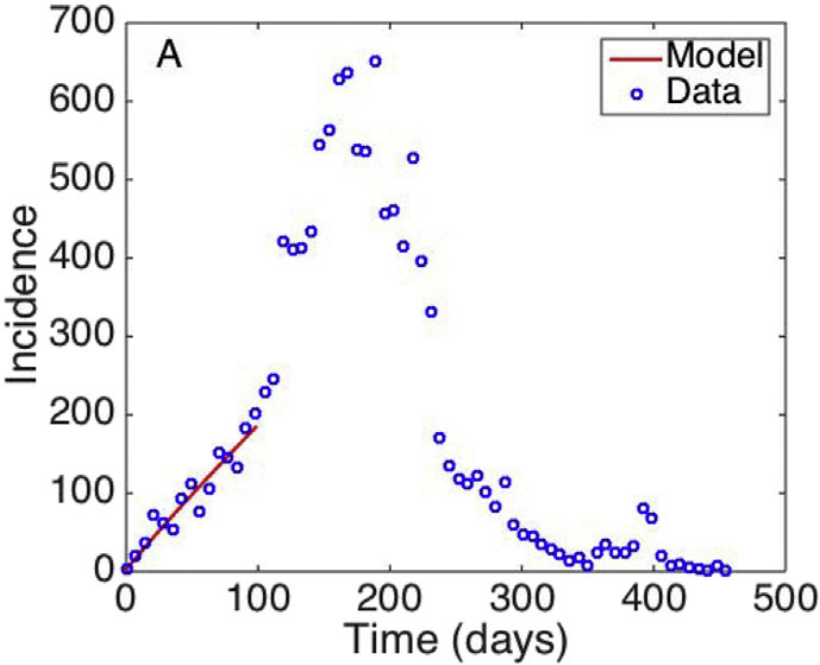
\includegraphics[width=.95\linewidth]{assets/DataR_zeroFitting}
    \end{center}
\end{frame}

\begin{frame}{Important Problems}
    \begin{textblock*}{50mm}(5mm, 25mm)
        \begin{itemize}
            \item
                Parameter estimation
            \item
                Control strategies modeling
            \item
                $\mathcal{R}_0$ definition in
             exotic dynamics: 
             Stochastic, Fractional, Functional
            \item
                Modeling plant and animal diseases
            \item
                Forecasting
        \end{itemize}
    \end{textblock*}
    \only<2>{
        \begin{textblock*}{60mm}(65mm, 27mm)
            \begin{yellowbox}{Objective:}
               Illustrate epidemic modeling ideas in 
               the formulation of an optimal 
               controlled model.
            \end{yellowbox}
        \end{textblock*}
    }
\end{frame}


